\section{Android Application}

In the pursuit of developing an Android application for the detection of road degradation, we encountered several challenges with the existing application. This section outlines the development process and improvements made to the application to meet our project requirements.



\subsection{Previous Application}
The original application was developed by Fabien, who is no longer part of the project team. This application was written in Kotlin, a language with which the team was not fully comfortable. One significant limitation was the difficulty in accessing the recorded data, as it required using Android Studio for data retrieval. Furthermore, the application lacked GPS data recording, which is crucial for our project's objectives. These limitations prompted the decision to start from scratch, redeveloping the application in Java and investing time in mastering Android Studio.

\begin{figure}[H]
    \centering
    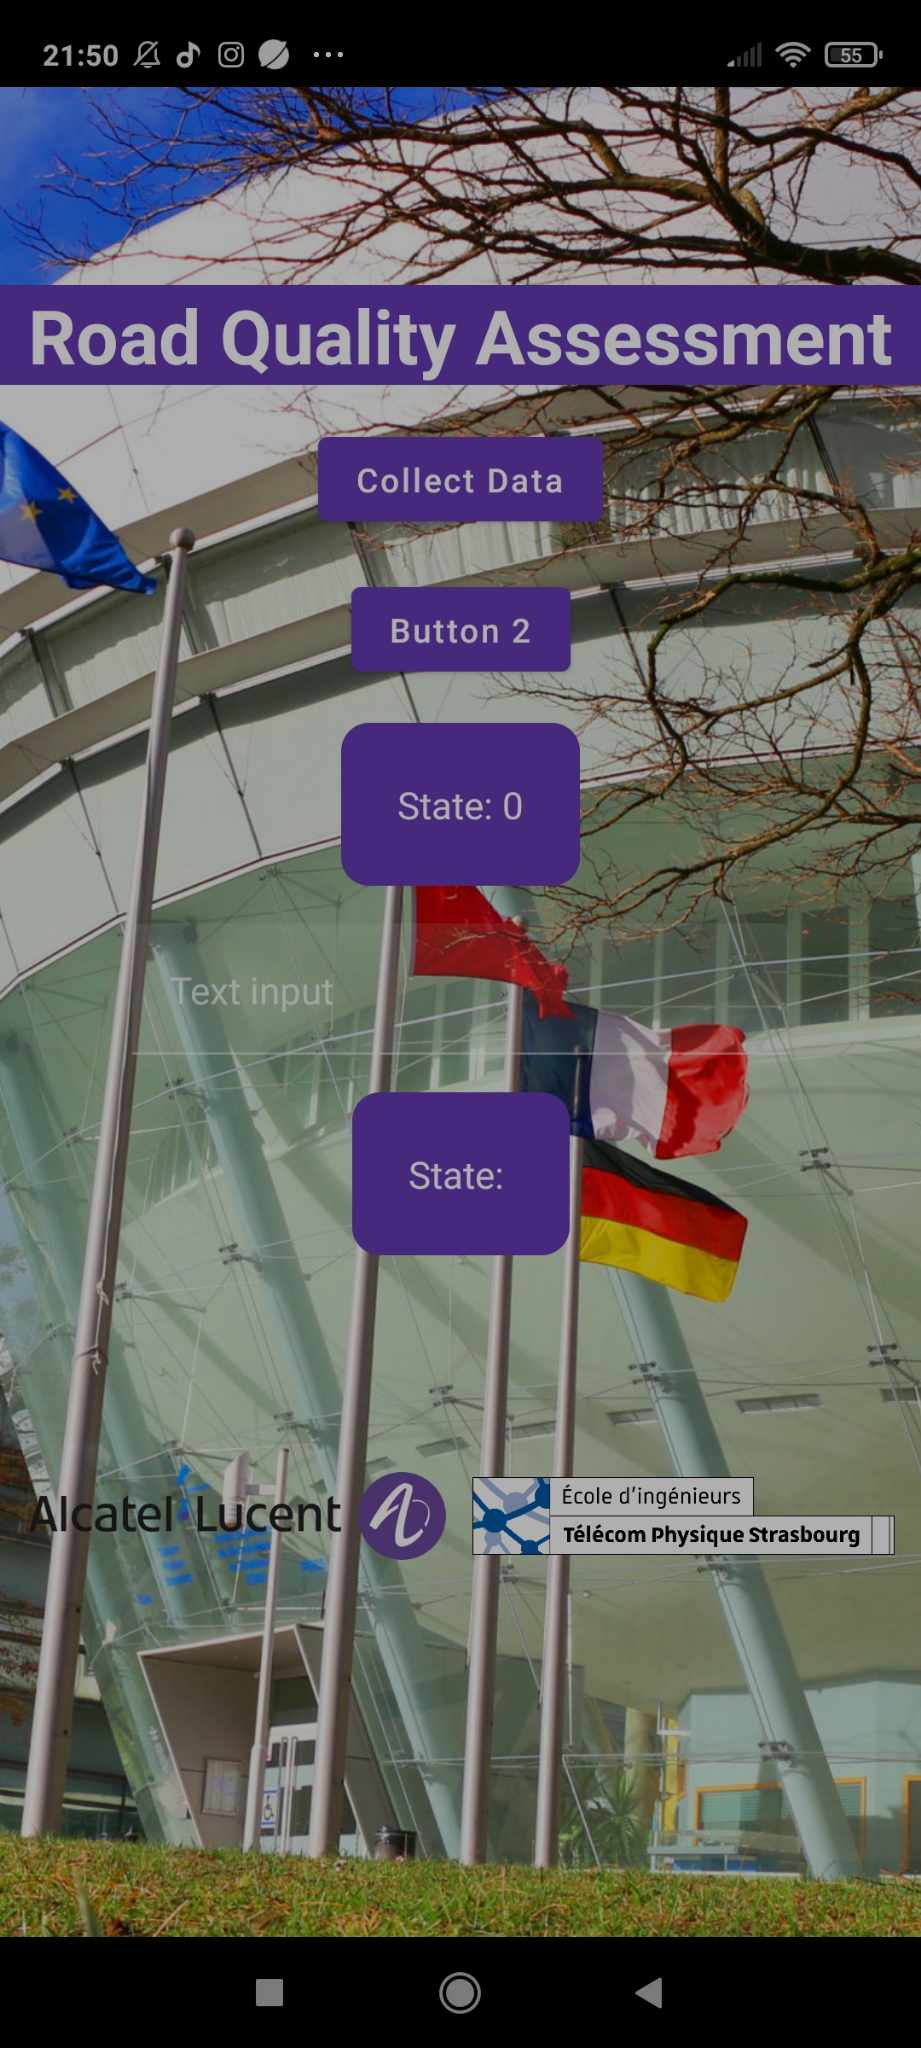
\includegraphics[width=0.3\linewidth]{ancienne.jpg}
    \caption{Previous Application}
    \label{fig:enter-label}
\end{figure}

\subsection{New Application Development}
With extensive research and the aid of tutorials, we successfully developed a new Android application tailored to our project requirements. The application now records both accelerometer data and GPS coordinates, ensuring that the data is readily accessible within the device's memory.

\begin{figure}[H]
    \centering
    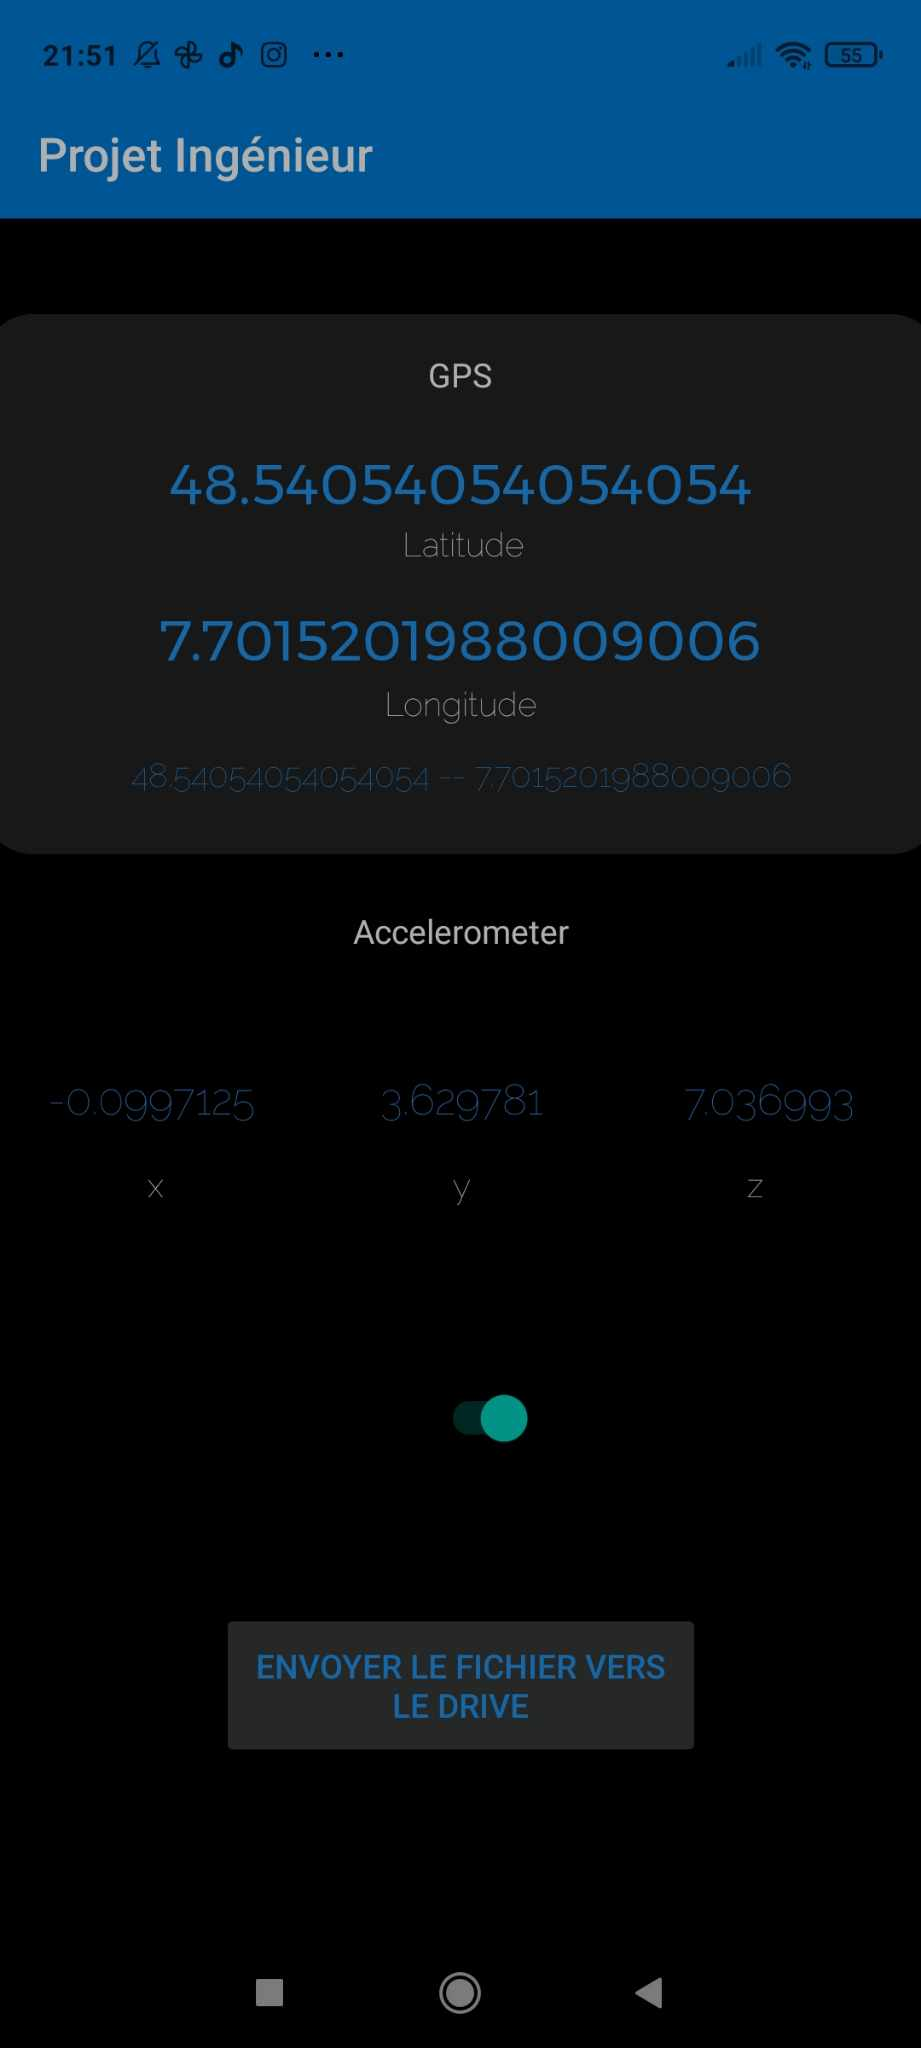
\includegraphics[width=0.3\linewidth]{nouvelle.jpg}
    \caption{New Application}
    \label{fig:enter-label}
\end{figure}

\subsection{Integration with Google Drive}
To facilitate the use of the recorded data with classification algorithms, we devised a solution to directly send the data file to Google Drive. This enables us to utilize the data within a Colab notebook or any other analysis tool that is compatible with Google Drive. The process involves integrating the application with the Google Drive API by using a Google API key.

\subsection{How It Works}
To use the application, follow these steps:

\begin{enumerate}
    \item Log in with your Google account credentials.
    \item Initiate data acquisition (the application allows pausing, and data is continuously displayed on the screen).
    \item Once data acquisition is complete, click on the "Send File to Drive" button to easily retrieve the data in CSV format.
\end{enumerate}

\subsection{Data Format}
The output file is named "MonFichierCSV.csv" and contains the following columns:

\begin{itemize}
    \item \texttt{ax}: Accelerometer x-axis data
    \item \texttt{ay}: Accelerometer y-axis data
    \item \texttt{az}: Accelerometer z-axis data
    \item \texttt{GPS\_lat}: Latitude data from GPS
    \item \texttt{GPS\_long}: Longitude data from GPS
\end{itemize}

\begin{figure}[H]
    \centering
    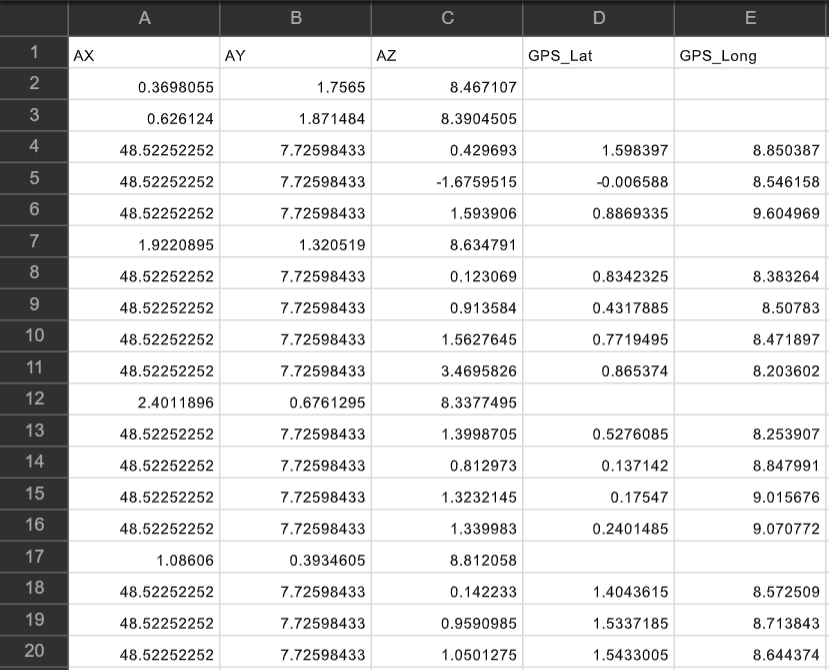
\includegraphics[width=0.5\linewidth]{csv.png}
    \caption{Few lines of the CSV file}
    \label{fig:enter-label}
\end{figure}

\subsection*{Limitations}
At present, one limitation of the application is that, since it is not validated by Google, only the holder of the API key can save the data file to Google Drive.

